Nous allons exploiter une idée toute simple à comprendre. Partons de la configuration gagnante pour trouver toutes les configurations obtenues en faisant un seul mouvement.
À partir des précédentes nouvelles configurations, nous recherchons ensuite d'autres configurations obtenues en faisant un second mouvement.
Ceci peut se résumer par l'arbre ci-dessous où une configuration $\mathcal{C}_1$ est reliée à une autre $\mathcal{C}_2$ uniquement si l'on peut passer de $\mathcal{C}_1$ à $\mathcal{C}_2$ en un seul mouvement. De plus, quand on descend dans l'arbre on ne garde que les nouvelles configurations.


\begin{center}
    \begin{tikzpicture}[
    rotate=0,
    level distance=1.5cm,
        level 1/.style={sibling distance=5cm},
        level 2/.style={sibling distance=2.25cm},
    ]
    \node{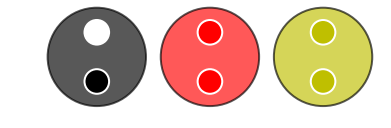
\includegraphics[scale=0.14]{content/optimal/tree_sol/moves/0.png}}
child{node{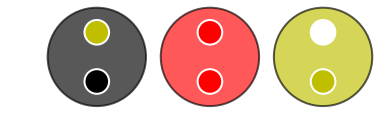
\includegraphics[scale=0.14]{content/optimal/tree_sol/moves/1.png}}
child{node{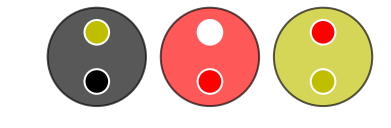
\includegraphics[scale=0.14]{content/optimal/tree_sol/moves/3.png}}}
child{node{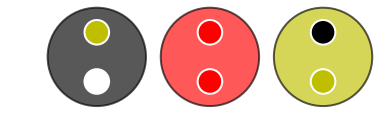
\includegraphics[scale=0.14]{content/optimal/tree_sol/moves/4.png}}}}
child{node{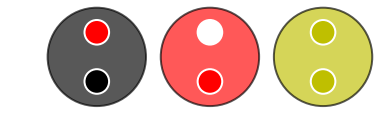
\includegraphics[scale=0.14]{content/optimal/tree_sol/moves/2.png}}
child{node{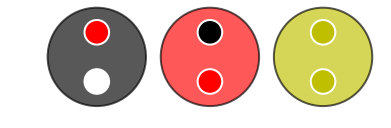
\includegraphics[scale=0.14]{content/optimal/tree_sol/moves/5.png}}}
child{node{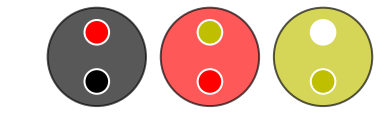
\includegraphics[scale=0.14]{content/optimal/tree_sol/moves/6.png}}}};
    \end{tikzpicture}
\end{center}



Avec un mouvement de plus, nous avons l'arbre ci-dessous (qui n'est pas symétrique : voir en bas à gauche).


\begin{center}
    \begin{tikzpicture}[
    rotate=0,
    level distance=1.5cm,
        level 1/.style={sibling distance=8.5cm},
        level 2/.style={sibling distance=4.75cm},
        level 3/.style={sibling distance=2cm},
    ]
    \node{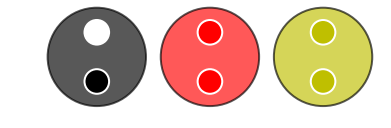
\includegraphics[scale=0.12]{content/optimal/tree_sol/moves/0.png}}
child{node{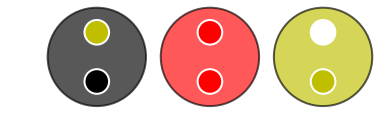
\includegraphics[scale=0.12]{content/optimal/tree_sol/moves/1.png}}
child{node{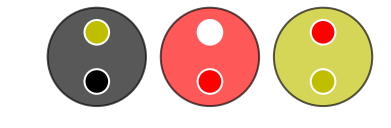
\includegraphics[scale=0.12]{content/optimal/tree_sol/moves/3.png}}
child{node{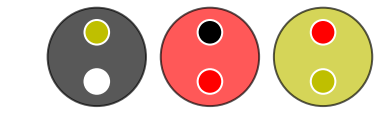
\includegraphics[scale=0.12]{content/optimal/tree_sol/moves/7.png}}}
child{node{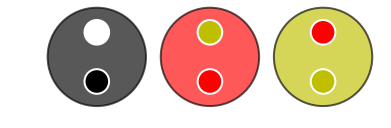
\includegraphics[scale=0.12]{content/optimal/tree_sol/moves/8.png}}}
child{node{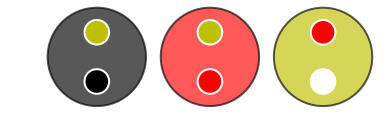
\includegraphics[scale=0.12]{content/optimal/tree_sol/moves/9.png}}}}
child{node{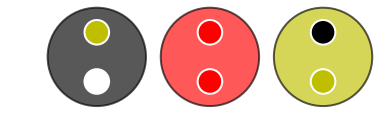
\includegraphics[scale=0.12]{content/optimal/tree_sol/moves/4.png}}
child{node{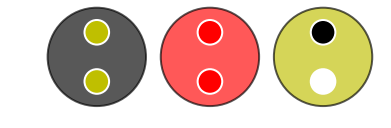
\includegraphics[scale=0.12]{content/optimal/tree_sol/moves/10.png}}}
child{node{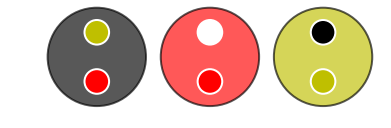
\includegraphics[scale=0.12]{content/optimal/tree_sol/moves/11.png}}}}}
child{node{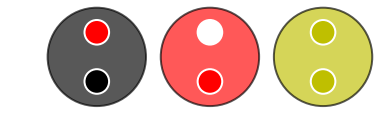
\includegraphics[scale=0.12]{content/optimal/tree_sol/moves/2.png}}
child{node{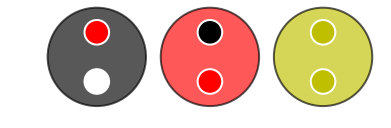
\includegraphics[scale=0.12]{content/optimal/tree_sol/moves/5.png}}
child{node{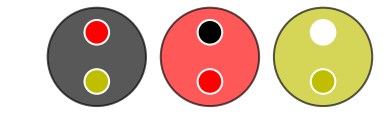
\includegraphics[scale=0.12]{content/optimal/tree_sol/moves/12.png}}}
child{node{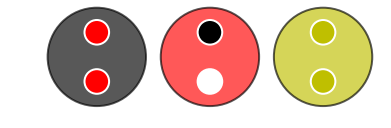
\includegraphics[scale=0.12]{content/optimal/tree_sol/moves/13.png}}}}
child{node{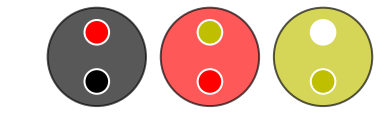
\includegraphics[scale=0.12]{content/optimal/tree_sol/moves/6.png}}
child{node{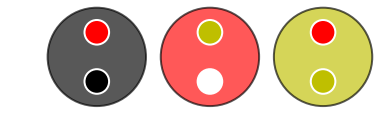
\includegraphics[scale=0.12]{content/optimal/tree_sol/moves/14.png}}}
child{node{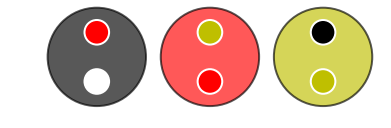
\includegraphics[scale=0.12]{content/optimal/tree_sol/moves/15.png}}}}};
    \end{tikzpicture}
\end{center}



Avec de la patience, ou grâce à un programme, on peut fabriquer l'arbre complet (vous le trouverez en annexe). Notons que pour un jeu à cinq bases, il y a tout de même $11\,010$ configurations (ceci est justifié en annexe), donc représenter l'arbre complet pour 5 bases sur une feuille A3, même avec l'aide d'un programme, ne sera pas possible. 


\medskip

Il est évident que la méthode que nous employons va finir par trouver toutes les configurations tout en nous indiquant une résolution proposant un minimum de coups à faire.
Il faut prendre garde que rien ne nous indique qu'il n'y a qu'une seule façon optimale de résoudre une configuration. En fait, il n'y a pas toujours unicité comme le montre la remarque n°1 juste après l'algorithme. 


\medskip

Notre démarche peut se traduire par l'algorithme ci-dessous où nous utilisons des dictionnaires qui sont des objets associant une valeur à une clé. Par exemple, \verb+mon_dico = {"un": 1, "deux": 2}+ admet pour clés \verb+"un"+ et \verb+"deux"+, et nous notons \verb+mon_dico<"un"> = 1+ la valeur associée à la clé \verb+"un"+.
Nous utilisons aussi $[ \,\, ]$ pour indiquer une liste vide prête à être remplie.


\bigskip

\begin{algo}
	\Data{une configuration quelconque de début de jeu}
	\Result{la solution gagnante (en utilisant le moins de déplacements possible)}
	\vspace{0.4em}
    \Begin{
		\vspace{0.4em}
		$\cal G$ désigne la configuration gagnante.
		\\
		\vspace{0.4em}
		\tcp{"L'arbre" sera construit sous forme d'un dictionnaire.}
		\tcp{\quad \textbullet{} les clés sont les configurations possibles.}
		\tcp{\quad \textbullet{} chaque valeur donne la liste des configurations à suivre pour gagner}
		\tcp{\phantom{\quad \textbullet{}} le plus rapidement possible (lecture de la liste de gauche à droite).}
		$\mathcal{A} \leftarrow \{ \mathcal{G} : [ \,\, ] \}$ 
		\\
		\vspace{0.4em}
		\tcp{Liste stockant les [n]ouvelles [c]onfigurations d'où partir.}
		$NC \leftarrow \big[ \, \mathcal{G} \, \big]$
		\\
		\vspace{0.4em}
		\While{$NC$ n'est pas vide}{
			\vspace{0.4em}
			$NC_{ap} \leftarrow [ \,\, ]$ va stocker les configurations d'où partir durant l'étape d'après.
			\\
			\vspace{0.4em}
			\ForEach{configuration $\mathcal{C}$ dans $NC$}{
				\ForEach{configuration $\mathcal{V}$ obtenue en un seul mouvement depuis $\mathcal{C}$}{
					\If{$\mathcal{V}$ n'est pas une clé de $\cal A$}{
						\vspace{0.4em}
						Ajouter $\mathcal{V}$ à $NC_{ap}$.
						\\
						\vspace{0.4em}
						$COUPS$ : liste obtenue en ajoutant $\mathcal{C}$ à gauche de la liste $\mathcal{A} \big\langle \mathcal{C} \big\rangle$.
						\\
						Ajouter $\mathcal{V}$ à $\mathcal{A}$ avec $\mathcal{A} \big\langle \mathcal{V} \big\rangle = COUPS$.
					}
				}
			}
			\vspace{0.4em}
			$NC \leftarrow NC_{ap}$
		}
		\vspace{0.4em}
		\tcp{Utilisation de l'arbre pour résoudre le jeu.}
		\vspace{0.4em}
		$\mathcal{C}_0$ : la configuration à résoudre.
		\\
		Obtenir successivement les configurations stockées de gauche à droite dans $\mathcal{A} \big\langle \mathcal{C}_0 \big\rangle$.
    }
\end{algo}


\medskip

\paragraph{Remarque n°1 :} \hspace{-1em} comme l'arbre construit  par l'algorithme \quote{tout connaître pour avancer vite} dépend de l'ordre dans lequel on explore les nouvelles possibilités, il y a peu de chances que l'on ait une solution optimale unique pour chaque configuration. L'exemple suivant montre qu'effectivement il n'y a pas unicité.

\vspace{-0.4em}
\begin{multicols}{2}
	\begin{center}   % [None, 0, 1, 2, 1, 2]
		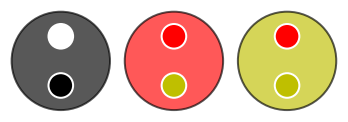
\includegraphics[scale=0.25]{content/optimal/tree_sol/no_unicity/sol_1/000.png}

		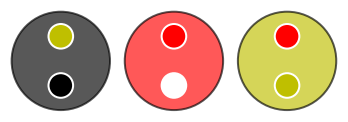
\includegraphics[scale=0.25]{content/optimal/tree_sol/no_unicity/sol_1/001.png}

		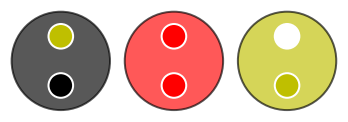
\includegraphics[scale=0.25]{content/optimal/tree_sol/no_unicity/sol_1/002.png}

		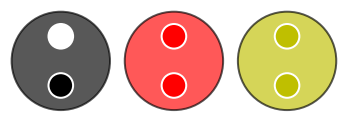
\includegraphics[scale=0.25]{content/optimal/tree_sol/no_unicity/sol_1/003.png}
	\end{center}

	\columnbreak
	\begin{center}   % SAME START
		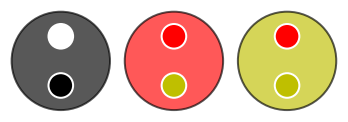
\includegraphics[scale=0.25]{content/optimal/tree_sol/no_unicity/sol_1/000.png}

				     % [1, 0, 1, 2, None, 2]
		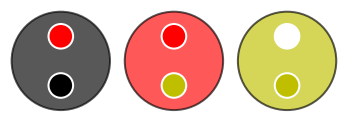
\includegraphics[scale=0.25]{content/optimal/tree_sol/no_unicity/sol_2/001.png}

				     % [1, 0, 1, None, 2, 2]
		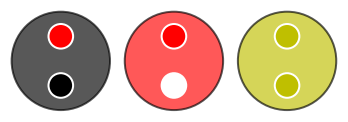
\includegraphics[scale=0.25]{content/optimal/tree_sol/no_unicity/sol_2/002.png}

				     % SAME END
		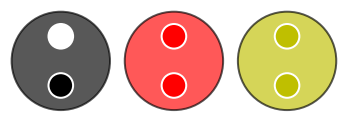
\includegraphics[scale=0.25]{content/optimal/tree_sol/no_unicity/sol_1/003.png}
	\end{center}
\end{multicols}

Ceci étant noté, si l'on visualise le jeu en cercle, et non plus en ligne, les deux solutions précédentes sont équivalentes puisque sur chaque ligne, la configuration de gauche et celle de droite sont dans le cercle symétriques par rapport à la base noire.
Autrement dit, la colonne de droite est obtenue à partir de celle de gauche en échangeant les couleurs rouges et jaunes, et aussi l'ordre des deux bases rouges et jaunes (ce qui est autorisé puisque l'on choisit un sens de parcours pour \quote{aplatir} le cercle).

\paragraph{Remarque n°2 :} \hspace{-1em} si l'on considère l'exemple donné dans la section précédente \quote{Où tentons-nous d'aller ?}, la méthode \quote{tout connaître pour avancer vite} propose exactement les 9 coups proposés pour illustrer certaines maladresses de l'algorithme \quote{on avance au mieux}


\paragraph{Remarque n°3 :} \hspace{-1em} l'algorithme \quote{tout connaître pour avancer vite}, bien que facile à programmer, est inutilisable par un humain dès le jeu à quatre bases qui permet d'avoir $480$ configurations différentes (voir l'annexe pour le calcul de cette valeur).
